\section{The website}
\label{sec:website}

This section describes the main technical characteristics of the website, and the technologies it is built with.
It starts with the notion of Single-page application, that is explained in {\sc subsection}~\ref{ssec:spa}.

\subsection{Single-page application}
\label{ssec:spa}

\url{www.konnektid.com} is a special kind of web application called Single-page application (\guillemotleft{} SPA \guillemotright{}).
This means that it loads one unique web page, and the totality of its necessary code, right from the start.
After that initial load, all of the presentation logic is handled by the client side, through JavaScript.
When the user interacts with the page, only affected parts of it are dynamically updated, without any server intervention.
The main goal of SPAs is to create a more fluid and responsive user experience, by avoiding page reloads.

There are various techniques and frameworks available for implementing SPAs.
Among them, Konnektid uses several that are described in {\sc subsection}~\ref{ssec:frameworks}.

\subsection{Frameworks and libraries}
\label{ssec:frameworks}

The website is principally coded in JavaScript, HTML and SCSS. It also features a certain number of frameworks and librairies: the main ones are described in the present section.

\subsubsection{ReactJS}
\label{sssec:react}

This is an open-source front-end JavaScript library, aiming at building user interfaces using encapsulated components. React implements a \guillemotleft{} virtual DOM \guillemotright{}, which is a quick representation of the actual DOM. It defines all the possible views for the page. When the application needs to be updated, a \textit{render()} method is called and returns the expected result, depending on the virtual DOM an the given data. There are two kinds of data for a React component:

\paragraph{The state} It is a set of internal data, that can only be updated by the component itself using the \textit{setState()}  method. If no data has been received yet, the component can define an initial state. All React components do not necessary have state: if they do, they are called \guillemotleft{} stateful \guillemotright{}, in opposition to \guillemotleft{} stateless \guillemotright{} for the others. When the state of a component changes, the rendered markup is automatically updated.

\paragraph{The props} These properties are passed down to the component by one of its parents, and can be accessed by calling \textit{this.props}. They cannot be modified by the component, but to avoid issues if not provided it is possible to define default values. The DOM is not re-rendered every time that the component gets new props; the developer has to write the call himself.

Although it is not mandatory, most developers (including the ones at Konnetid) use React with JSX, a preprocessor step that adds XML-like syntax to JavaScript. It makes the code easier to debug, and usually faster thanks to the optimization performed during compilation. {\sc figure}~\ref{fig:jsx} demonstrates how much code is simplified with JSX.

\begin{figure}[H]
    \centering
    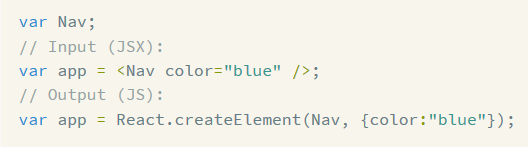
\includegraphics[scale=0.9]{figure/jsx.png}
    \caption{An example of JSX code and its JavaScript output.}
    \label{fig:jsx}
\end{figure}

\subsubsection{Node.js}
\label{sssec:node}

Konnektid's server-side code is mostly based on Node.js, an event-driven JavaScript runtime. It is particularly efficient because it uses Google Chrome's V8 engine, an open-source tool that is able to quickly analyze and execute JavaScript code.

Another reason why Node.js is very fast is its non-blocking code architecture. This means that the program does not need to wait to finish an action before launching a new one. Instead, when starting a request, a callback function is assciated to it and will be fired as soon as the request is achieved. These notifications allow the system to keep working on other tasks in the meantime, as illustrated on {\sc figure}~\ref{fig:callback}.

\begin{figure}[H]
    \centering
    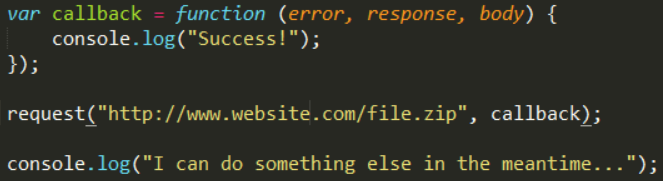
\includegraphics[scale=0.8]{figure/callback.png}
    \caption{An example of non-blocking code with a callback function.}
    \label{fig:callback}
\end{figure}

Another strong suit of Node.js is its package ecosystem, npm (\url{https://www.npmjs.com/}), that is considered to be the largest ecosystem of open source libraries in the world.

\subsubsection{Redux}
\label{sssec:redux}

Redux is a predictable container for JavaScript applications, that stocks the whole state into one object tree called \guillemotleft{} store \guillemotright{}. This state is read-only: the only way to change it is to emit an \guillemotleft{} action \guillemotright{}, i.e. an object describing what happened and eventually passing down some data. To specify how the state tree is transformed by actions, Redux uses \guillemotleft{} reducers \guillemotright{}. They are pure functions that take the previous state and an action, and return the next state in a new object. This behaviour is summarized on {\sc figure}~\ref{fig:reduxSumup}.

\begin{figure}[H]
    \centering
    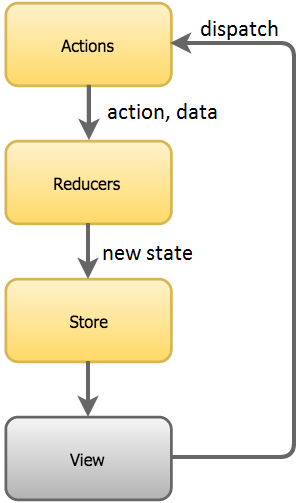
\includegraphics[scale=0.7]{figure/redux_flow.png}
    \caption{A simplified diagram of how Redux works.}
    \label{fig:reduxSumup}
\end{figure}

\subsubsection{GraphQL}
\label{sssec:grqphql}

To retrieve data from its database, Konnektid uses the GraphQL type system, to interpret queries. To be understood by GraphQL, these queries must respect a specific format illustrated on the left side of {\sc figure}~\ref{fig:query}. The provided result is an object, containing all the required fields, as visible on the right side of {\sc figure}~\ref{fig:query}. 

\begin{figure}[H]
    \centering
    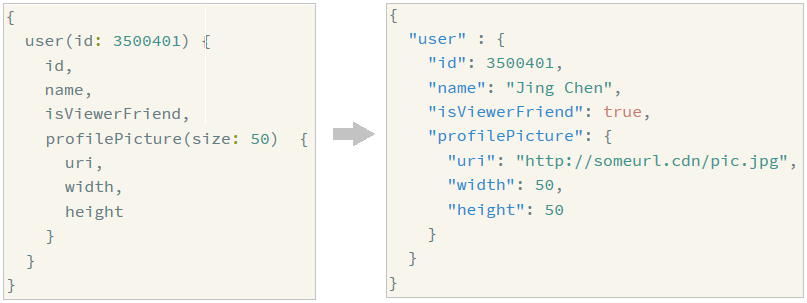
\includegraphics[scale=0.8]{figure/query.png}
    \caption{An example of GraphQL query and its result.}
    \label{fig:query}
\end{figure}

It is noticeable that the query is shaped just like the data it returns. This makes it more natural to write and also to understand.
Another particularity of GraphQL is that queries are encoded in the client rather than the server. This allows to return exactly what a client asks for and no more.

Now that the main technologies have been introduced, it is time to start {\sc section}~\ref{sec:github} that describes the development process and the use of Github inside the Konnekid team.